%%%%%%%%%%%%%%%%%%%%%%%%%%%%%%%%%%%%%%%%%
% Dreuw & Deselaer's Poster
% LaTeX Template
% Version 2.0 (February 18, 2023)
%
% This template originates from:
% https://www.LaTeXTemplates.com
%
% Authors:
% Vel (vel@latextemplates.com)
% Philippe Dreuw and Thomas Deselaers (https://github.com/deselaers/latex-beamerposter)
%
% License:
% CC BY-NC-SA 4.0 (https://creativecommons.org/licenses/by-nc-sa/4.0/)
%
% NOTE: The bibliography needs to be compiled using the bibtex engine.
%
%%%%%%%%%%%%%%%%%%%%%%%%%%%%%%%%%%%%%%%%%

%----------------------------------------------------------------------------------------
%	PACKAGES AND OTHER DOCUMENT CONFIGURATIONS
%----------------------------------------------------------------------------------------

\documentclass{beamer} % Use the beamer base class

\usepackage{bm}

\usepackage[
	orientation=portrait, % Portrait orientation
	size=a0, % Paper size
	scale=1.21, % Scale, it's important to adjust this so your content fits nicely in the template
]{beamerposter} % Use the beamerposter package to create the layout

\usetheme{I6pd2} % Use the I6pd2 theme supplied with this template

\usepackage{changepage} % Required for temporarily indenting text blocks

\usepackage{amsmath,amsthm,amssymb,latexsym} % For including math equations, theorems, symbols, etc

\usepackage{gfsdidot} % Use the GFS Didot font

\usepackage{booktabs} % Top and bottom rules for tables

\definecolor{hexagram}{RGB}{2, 235, 239}
\definecolor{hexagram1}{RGB}{255, 0, 0}
\definecolor{hexagram2}{RGB}{106, 188, 68}

\graphicspath{{Figures/}} % Location of figure images

%----------------------------------------------------------------------------------------
%	TITLE SECTION
%----------------------------------------------------------------------------------------

\title{\LARGE The SIR metapopulation model in a temporal commuting network} % Poster title

\author{*Gabriel F. Costa$^1$, Matheus M. G. Correia$^2$, Leonardo B. L. Santos$^3$, Vander L. S. Freitas$^4$} % Author(s)

\institute{\textsuperscript{1}Department of Physics, Federal University of Ouro Preto, Ouro Preto, Brazil, \textsuperscript{2} National Institute for Space Research, São José dos Campos, Brazil, \textsuperscript{3} National Center for Monitoring and Early Warning of Natural Disasters (CEMADEN), São José dos Campos, São Paulo, Brazil, \textsuperscript{4} Department of Computing, Federal University of Ouro Preto, Ouro Preto, Brazil.} % Institution(s)

%----------------------------------------------------------------------------------------
%	FOOTER TEXT
%----------------------------------------------------------------------------------------

\newcommand{\leftfoot}{https://csilab.ufop.br/} % Left footer text

\newcommand{\rightfoot}{https://github.com/gabrielxcosta/Simulation-of-epidemiological-models-in-temporal-mobility-networks} % Right footer text

%\setbeamertemplate{footline}{} % Uncomment this line to hide the footer

%----------------------------------------------------------------------------------------

\begin{document}

\begin{frame}[t] % The whole poster is enclosed in one beamer frame, the [t] parameter aligns everything to the top

\begin{columns}[t] % Begin multi-column layout, the [t] parameter aligns each column's content to the top

\begin{column}{0.02\textwidth}\end{column} % Empty column for horizontal whitespace

\begin{column}{0.465\textwidth} % Start the first content column

%----------------------------------------------------------------------------------------
%	OBJECTIVES
%----------------------------------------------------------------------------------------

\begin{block}{Research objectives}
	\begin{enumerate}
		\item Simulate the metapopulation SIR model in temporal mobility networks.
		\item Compare results obtained from dynamic networks and static versions.
		\item Quantify the differences between the simulated dynamics in the temporal network and its static version.
        \item Investigate the tolerance in changing the network's time resolution in relation to its more refined version.
        \item Analyze the correspondences between the changes in the dynamics with the topological changes of the network, in time.
	\end{enumerate}
\end{block}

%----------------------------------------------------------------------------------------
%	INTRODUCTION
%----------------------------------------------------------------------------------------
            
\begin{block}{Introduction}

	\textbf{Networks} \\
    A network is a set of interconnected elements $^{[4]}$. In graph theory and network science, networks are represented by a set of nodes interconnected by connections (or edges). Networks are a powerful way to represent and study complex systems in many areas, such as biology, sociology, technology, transportation, among others.

    \bigskip % Vertical whitespace

    \begin{figure}[h!]
		\centering % Horizontally center
		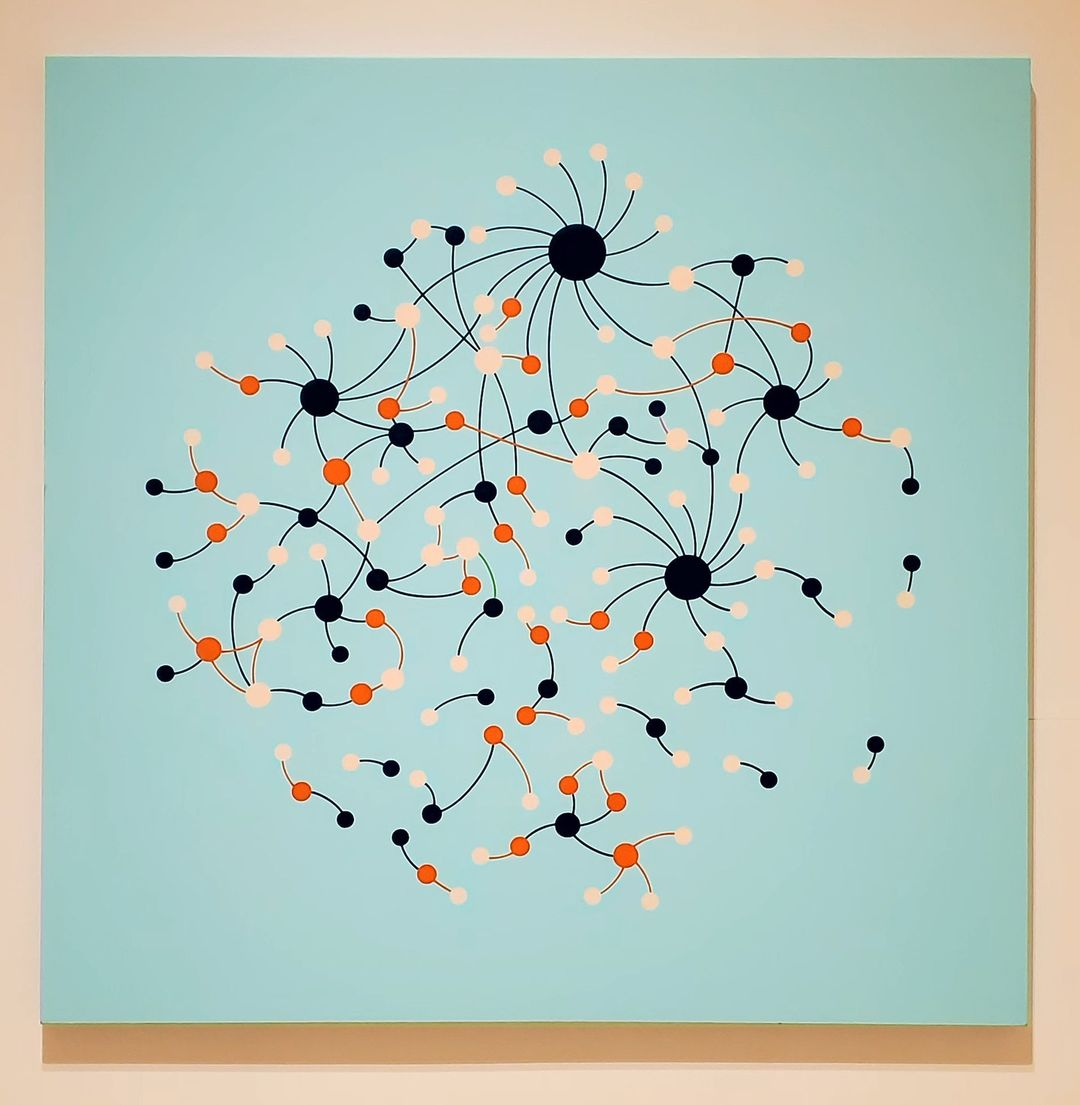
\includegraphics[width=0.40\linewidth]{network.jpg}
		\caption{BarabasiLAB Art - Museum of Modern Art, MOMA. Source: Postmasters, \url{https://www.postmastersart.com}.}
	\end{figure}
	
	\bigskip % Vertical whitespace

    \textbf{SIR model}

    The SIR model is a widely used mathematical framework for modeling and analyzing epidemics. It divides the population into three main groups: \textcolor{hexagram}{\textbf{susceptible (S)}}, \textcolor{hexagram1}{\textbf{infected (I)}}, and  \textcolor{hexagram2}{\textbf{recovered (R)}}. The model describes the spread of a disease over time, taking into account the rates of infection ($\boldsymbol{\beta}$), recovery ($\boldsymbol{\gamma}$), and contact between individuals.

    \bigskip

    \begin{figure}[h!]
		\centering % Horizontally center
		
\includegraphics[width=0.54\linewidth]{SIRmodel.png}
		\caption{SIR schematic diagram.} 
	\end{figure}

    \bigskip
    
    The SIR model is a simple but powerful approach that can be used to simulate different scenarios of disease spread. For example, the model can be used to simulate the effects of different vaccination rates, contact tracing strategies, and quarantine policies.

    \bigskip
    
    The SIR model has been used to study a wide range of diseases, including measles, influenza, and COVID-19. The model has helped to inform public health policy and practice, and it has been used to develop new strategies for preventing and controlling the spread of disease.

    \bigskip
    
    The ordinary SIR model for a metapopulation with $N$ hosts:
    
    \begin{center}
    \begin{equation}
    \begin{cases}
        \frac{dS}{dt} = -\frac{{\boldsymbol{\beta}} S I}{N}, \\
        
        \frac{dI}{dt} = \frac{{\boldsymbol{\beta}} S I}{N} - \gamma I, \\
        
        \frac{dR}{dt} = \gamma I.
    \end{cases}
    \end{equation}
    \end{center}
    
    \bigskip
	
	\textbf{Metapopulations} \\
    Metapopulation models represent geographically isolated host populations connected through movement. Assuming \textbf{homogeneous mixing} within local contexts, individuals within each population have random and equally probable contacts. Populations remain stable over time and can be calibrated using census data.

    \bigskip
    
    Disease transmission is assumed to be entirely local, with hosts from different subpopulations coming into contact only if they travel to the same location. 

    \bigskip
    
    \begin{figure}[h!]
        \centering % Horizontally center
        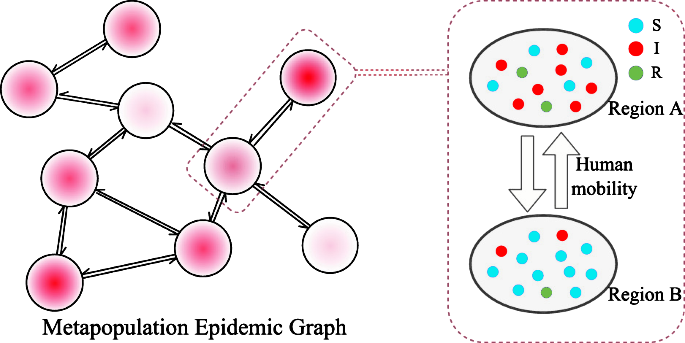
\includegraphics[width=0.47\linewidth]{MetapopSIR.png}
        \caption{SIR model in a metapopulation network.}
    \end{figure}
\end{block}

\end{column}

\begin{column}{0.03\textwidth}\end{column} % Empty column for horizontal whitespace
 
\begin{column}{0.465\textwidth} % Start the second content column

%----------------------------------------------------------------------------------------
%	CONCLUSIONS
%----------------------------------------------------------------------------------------

\begin{block}{Methodology}
    
    \textbf{Mobility and geographical data}

    We utilized the \textbf{Baidu Mobility Data} $^{[1]}$ from Jan-Feb 2020, before the official COVID-19 pandemic declaration. This dataset tracks daily movements between 340 Chinese cities $^{[3]}$.

    \bigskip
    
    The dataset includes two \textbf{adjacency matrices} for input and output streams. The input matrix shows the percentage of people moving from node $i$ to node $j$, with node $j$ representing the sum of all other entries. The output matrix behaves similarly. Each node has up to 100 neighbors.

    \bigskip
    
    The adjacency matrix of a directed network with $N$ nodes is an $N \times N$ matrix. Its elements, denoted as $A_{i,j}$, are set to $1$ if there is a directed link from node $j$ to node $i$, and $0$ if nodes $i$ and $j$ are not connected:

    \begin{center}
    \begin{equation}
    A_{i, j} = \begin{bmatrix}
    a_{1, 1} & a_{1, 2} & \cdots & a_{1, N} \\
    a_{2, 1} & a_{2, 2} & \cdots & a_{2, N} \\
    \vdots & \vdots & \ddots & \vdots \\
    a_{N, 1} & a_{N, 2} & \cdots & a_{N, N} \\
    \end{bmatrix}.
    \end{equation}
    \end{center}

    \bigskip
    
    \textbf{Host movement models}
    
    Host movement models are utilized to simulate the movement of hosts within a metapopulation network. These models can be adapted to represent human mobility by tracking individuals movements between different locations or nodes. \textbf{Eulerian} and \textbf{Lagrangian} movement models are the two most commonly used classes of such models.

    \bigskip

    We specifically employed the Eulerian movement model $^{[2]}$, which describes the \textbf{diffusion} of hosts among metapopulation, with the following set of differential equations:

    \bigskip

    \begin{center}
    \begin{equation}
    \frac{dN_{i}}{dt} = -\sum_{j=1}^{K} f_{i, j} N_{i} + \sum_{j=1}^{K} f_{j, i} N_{j},
    \end{equation}
    \end{center}

    $N_{i}$ represents the number of hosts currently located at site $i$, and $K$ denotes the total number of populations. The term $f_{i, j}$ corresponds to the rate (our adjacency matrix here will correspond of $NxN$ matrix of travel rates) at which hosts move from site $i$ to site $j$, with $f_{i, j}$ accounting for movement within the same population. The model requires a total of $K (K - 1)$ parameters for a complete specification.

    The total number of hosts remains constant over time:
    \begin{center}
    \begin{equation}
        N = \sum_{i=1}^{K} N_{i}.
    \end{equation}
    \end{center}

    Combining SIR model with Eulerian model, we obtain an analogous set of $3K$ equations, for $K$ subpopulations (nodes):

    \begin{equation}
    \large
    \begin{cases}
        \frac{dS_{i}}{dt} = -\beta_{i} \frac{S_{i}I_{i}}{N_{i}} -\sum_{j=1}^{K} f_{i, j} S_{i} + \sum_{j=1}^{K} f_{j, i} S_{j}, \\
        \frac{dI_{i}}{dt} = \beta_{i} \frac{S_{i}I_{i}}{N_{i}} - \gamma I_{i} -\sum_{j=1}^{K} f_{i, j} I_{i} + \sum_{j=1}^{K} f_{j, i} I_{j}, \\
        \frac{dR_{i}}{dt} = \gamma I_{i} -\sum_{j=1}^{K} f_{i, j} R_{i} + \sum_{j=1}^{K} f_{j, i} R_{j}.
    \end{cases}
    \end{equation}

    
\end{block}

\begin{block}{Conclusion}
This project is currently a work in progress. We have successfully accomplished objective number one, and our focus has now shifted to objective number two. Throughout the course of our work, we encountered the formidable challenge of sourcing relevant temporal mobility data from national and international surveys, which consumed a significant amount of our research time.
\end{block}

%----------------------------------------------------------------------------------------
%	REFERENCES
%----------------------------------------------------------------------------------------

\begin{block}{References}
    \small
	$^{[1]}$ China Data Lab. \textit{Baidu Mobility Data}, 2020. \\
    $^{[2]}$ Daniel T. Citron, Carlos A. Guerra, Andrew J. Dolgert, Sean L. Wu, John M. Henry, Héctor M. Sánchez C., and David L. Smith. \textit{Comparing metapopulation dynamics of infectious diseases under different models of human movement}, 2021. \\
    $^{[3]}$ Vander L. S. Freitas, Leonardo B. L. Santos, Ming Tang, Yong Zou, Elbert E. N. Macau. \textit{The effects of COVID-19 on Chinese commuting patterns in early 2020}, 2022. \\
    $^{[4]}$ A. L. Barabási. \textit{Network Science}, 2016.
    
    
\end{block}

%----------------------------------------------------------------------------------------
%	ACKNOWLEDGEMENTS
%----------------------------------------------------------------------------------------

\begin{block}{Acknowledgements}
We would like to thank \textbf{CNPq} and \textbf{Universidade Federal de Ouro Preto}, for their financial support.
\end{block}

%----------------------------------------------------------------------------------------
%	CONTACT INFORMATION
%----------------------------------------------------------------------------------------

\setbeamercolor{block title}{fg=black, bg=taorange} % Change the block title color

%----------------------------------------------------------------------------------------

\end{column} % End of the second column

\begin{column}{0.02\textwidth}\end{column} % Empty column for horizontal whitespace

\end{columns} % End of all the columns in the poster

\end{frame} % End of the enclosing frame

%----------------------------------------------------------------------------------------

\end{document}
